\chapter{Ungleichungen}

Autor: Marc Mittner

\section{Definition}

Eine Ungleichung stellt eine Ordnung zweier mathematischer Objekte dar. Ungleichungen werden bezüglich der Anzahl der Variablen und der Potenz, in der die Variablen auftreten, unterschieden. Dabei varriiert je nach Typ der Ungleichung das Lösungsverfahren.

\section{Äquivalenzumformung von Ungleichungen}

Zur Umformung von Ungleichungen sind folgende Operationen zulässig:
\begin{itemize}
\item Addition einer Zahl \textit{$ a  \in \mathbb{R} $ } auf beiden Seiten.
\item Subtraktion einer Zahl \textit{$ a  \in \mathbb{R} $ } auf beiden Seiten.
\item {Multiplikation mit einer Zahl \textit{$ a \in \mathbb{R} $ , $ a > 0 $} auf beiden Seiten.}
\item {Multiplikation mit einer Zahl \textit{$ a \in \mathbb{R} $ , $ a < 0 $} auf beiden Seiten. Dabei ist zu beachten, dass das Ordnungszeichen umgedreht wird!}
\item {Division durch eine Zahl \textit{$ a \in \mathbb{R} $ , $ a > 0 $ } auf beiden Seiten.} 
\item {Division durch Zahl \textit{$ a \in \mathbb{R} $ , $ a < 0 $} auf beiden Seiten. Dabei ist zu beachten, dass das Ordnungszeichen umgedreht wird!}
\item Bei Ziehen der Quadratwurzel muss darauf geachtet werden, dass die Ungleichung in zwei Teile zerfällt:
\[x^2 \ < \ a^2 ~~~~~~~~~ \Leftrightarrow \]
\[ -a \ < \ x \ < a ~~~ \Leftrightarrow \]
\[ |x| \ < \ a \]
(siehe Beispiel bei quadratischen Ungleichungen).
\end{itemize}
Änderung der Ordnungszeichen bei Multiplikation / Division mit einer Zahl $ a \ < \ 0 $:
\begin{itemize}
\item $ < $ wird zu $ > $ ~~~,~~~ $ > $ wird zu $ < $
\item $ \leq $ wird zu $ \geq $ ~~~,~~~ $ \geq $ wird zu $ \leq $
\item Die Zeichen "`$ = $"' und "`$ \neq $"' bleiben erhalten.
\end{itemize}
Nicht erlaubt sind folgende Umformungen:
\begin{itemize}
\item beidseitige Multiplikation mit 0
\item beidseitige Division durch 0
\item beidseitiges Quadrieren 
\end{itemize}
\section{Lineare Ungleichungen}

Eine lineare Ungleichung ist eine Ungleichung, in der die Variable nur in der ersten Potenz enthalten ist. Jede lineare Ungleichung kann in die Form \\ 
\[ax \ + \ b \ > \ c \] bzw. 
\[ax \ + \ b \ \geq c \] bzw. 
\[ax \ + \ b \ \neq c \] 
zusammengefasst werden.

Zur Lösung einer linearen Ungleichung wird die Variable isoliert:

Beispiel:
\[3 - 4x - 13 + 2x - 3x + 12 \leq 5 \\ Zusammenfassen \]
\[-5 x \ + \ 2 \ \leq \ 5\\ |-2 \]
\[-5x \ \leq \ 3 \\ ~~~~~~~~~~~~| \div (-5) \]
\[ x \ \geq \ - \frac 3 5\]

\Large \bfseries {Graphische Darstellung des Lösungsbereichs}
\mdseries 	\normalsize
\begin{center}
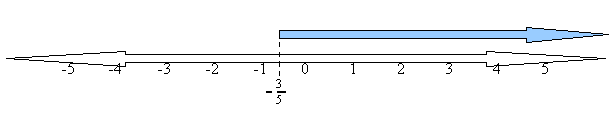
\includegraphics[width=0.8\textwidth]{img/LBer1.png}
\end{center}

Allgemein:
\[ax \ + \ b \ \leq \ c \\ |-b \]
\[ax \ \leq \ c \ - \ b \\ ~~~~~~~~~~~~~|\div a ~(a \ > \ 0) \]
\[x \leq \frac {c \ - \ b} a\]

\section{Quadratische Ungleichungen}

Bei quadratischen Ungleichungen können Variablen auch in der zweiten Potenz
auftreten. Jede quadratische Ungleichung kann in die Form \\
\[x^2 \ + \ px \ + \ q \ > \ r \]
bzw. 
\[x^2 \ + \ px \ + \ q \ \geq \ r \]
bzw.
\[x^2 \ + \ px \ + \ q \ \neq \ r \]
zusammengefasst werden.

Zur Lösung wird das Verfahren der quadratischen Ergänzung verwendet.
Bei diesem Verfahren wird zur normierten Form der quadratischen Ungleichung $ x^2 \ + \ px \ + \ q \ > \ r $ der Teil $ x^2 \ + \ px $ zu einer binomischen Formel erweitert.

%\newpage
Allgemein:
\[x^2 \ + \ px \ + \ q \ < \ r \\ ~~~~~~~~~~~~~~~~~~~~~|-q \] 
Quadratische Ergänzung:
\[x^2 \ + \ px \ < \ r \ - \ q \\ ~~~~~~~~~~~~~~~~~~~~~~~~~~~~|+ \left(\frac 1 2 p \right)^2\]
\[x^2 \ + \ px \ + \ \left(\frac 1 2 p \right)^2 \ < \ r \ - \ q \ + \left(\frac 1 2 p \right)^2 \\ Binom \]
\[\left(x \ + \ \frac 1 2 p \right)^2 \ < \ r \ - \ q \ + \left(\frac 1 2 p \right)^2\]
\[|x \ + \ \frac 1 2 p| \ < \ \sqrt{ r \ - \ q \ + \ \left(\frac 1 2 p \right)^2}\]
Daraus folgen die beiden Lösungen:
\[x_1 \ < \ \sqrt{r  \ - \ q \ + \ \left(\frac 1 2 p \right)^2} \ - \ \frac 1 2 p\]
\[x_2 \ > \ -\sqrt{r \ - \ q \ + \ \left(\frac 1 2 p \right)^2} \ - \ \frac 1 2 p\]
Somit erhält man die p-q-Formel für quadratische Gleichungen in normierter Form ($ r = 0 $):
\[x_{1,2} \ = \ - \frac p 2 \ \pm \ \sqrt{ \left( \frac p 2 \right)^2 \ - \ q}\]

Beispiel:
\[5x^2 + 12 - 12x - 3x^2 \geq 26 \\ Zusammenfassen\]
\[2x^2 \ - \ 12x \ + \ 12 \ \geq \ 26 \\Normieren \]
\[x^2 \ - \ 6x \ + \ 6 \ \geq \ 13 \\ |-6 \]
Quadratische Ergänzung:
\[x^2 \ - \ 6x \ \geq \ 7 \\ ~~~~~~~~~~|+9\]
\[x^2 \ - \ 6x \ + \ 9 \ \geq \ 16 \\ 2. binom. Formel\]
\[(x \ - \ 3)^2 \ \geq \ 16\]
Die Ungleichung zerfällt in zwei Teile:
\[|x \ - \ 3| \ \geq \ 4 \]
1. Fall:
\[x_1 \ - \ 3 \ \geq 4\]
\[x_1 \ \geq \ 7\]
2. Fall: 
\[-x_2 \ + \ 3 \ \geq \ 4\]
\[x_2 \ \leq \ -1\]

\minisec{Graphische Darstellung des Lösungsbereichs}
\mdseries 	\normalsize
\begin{center}
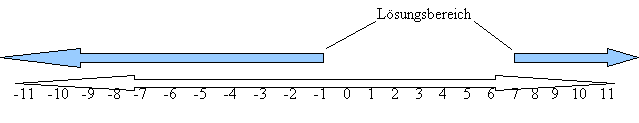
\includegraphics[width=0.8\textwidth]{img/LBer2.png}
\end{center}

\section{Ungleichungen höherer Ordnung}

Zum Lösen von Ungleichungen höherer Ordnung eignet sich wegen der Komplexität der Gleichungen meist nur die Darstellung der Gleichung als Produkt in der Form: 
\[(x \ - \ a_1)(x \ - \ a_2)...(x \ - \ a_n) > 0 \]
Die analytische Berechnung der Nullstellen ist aber nicht immer möglich. Lediglich bei Ungleichungen der Ordnung drei ist diese Faktorisierung noch praktikabel.

\section{Bruchungleichungen}

Bei Bruchungleichungen ist darauf zu achten, dass zuerst der Definitionsbereich festgestellt werden muss, da eine Division durch Null nicht zulässig ist. Dazu werden alle Belegungen der Variablen, die eine solche Division verursachen würden, aus dem Definitionsbereich entnommen.

\subsection{Lösen von Bruchungleichungen}

Zum Lösen von Bruchungleichungen benutzt man folgende Vorgehensweise:
\begin{itemize}
\item Multiplikation beider Seiten mit dem Hauptnenner
\item Ausmultiplizieren
\item Lösen der entstehenden quadratischen Ungleichung
\end{itemize}

\subsection{Beispiel}

\[ \frac{(3x \ - \ 2)} {(x \ + \ 2)} + \frac{(2 \ + \ 5x)} {(x^2 \ - \ 4)} \ \leq \ \frac{(x \ + \ 3)} {(x \ - \ 2)}\]
Definitionsbereich \ $ D \ = \ \mathbb{R} \setminus \lbrace -2 , +2 \rbrace $
Multiplikation mit dem Hauptnenner $ (x \ + \ 2)(x \ - \ 2) \ = \ (x^2 \ - \ 4) $:
\[ \frac{(3x \ - \ 2)} {(x \ + \ 2)} \cdot (x^2 \ - \ 4) + \frac {(2 \ + \ 5x)} {(x^2 \ - \ 4)} \cdot (x^2 \ - \ 4) \ \leq \ \frac{(x \ + \ 3)} {(x \ - \ 2)} \cdot (x^2 \ - \ 4)\]
\[(3x \ - \ 2)(x \ - \ 2) + \ 2 \ + \ 5x \ \leq \ (x \ + \ 3)(x \ + \ 2)\]
Ausmultiplizieren:
\[3x^2 \ - \ 8x \ + \ 4 \ + \ 2 \ + \ 5x \ \leq \ x^2 \ + \ 5x \ + \ 6\]
Lösen der entstandenen quadratischen Gleichung:
\[ 2x^2 \ - \ 8x \ \leq \ 0 \]
\[ x^2 \ - \ 4x) \ \leq \ 0 \]
\[ x^2 \ - \ 4 x \ + \ 4 \ \leq \ 4 \]
\[ |x \ - \ 2| \ \leq \ 2 \]
\[x \ \leq \ 4 \]
\[ x \ \geq \ 0 \]
Lösung für die Ungleichung sind somit alle $ x $ mit $ 0 \ \leq x \ \leq \ 4 $ außer $ x \ = \ 2 $, da diese Belegung nicht im Definitions- und somit auch nicht im Lösungsbereich liegt.
\[L \ = \ \lbrace x \in \mathbb{R} \ | \ 0 \ \leq x \ \leq \ 4 \rbrace \setminus \lbrace 2 \rbrace\]

\minisec{Graphische Darstellung des Lösungsbereichs}
%\mdseries 	\normalsize
\begin{center}
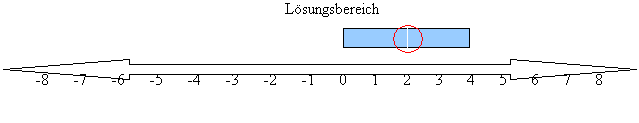
\includegraphics[width=0.8\textwidth]{img/LBer3.png}
\end{center}

\section{Ungleichungen mit mehreren Variablen}

Bei Ungleichungen mit mehreren Variablen ist der Lösungsbereich nicht mehr ein-, sondern mehrdimensional. Die Dimension nimmt mit der Anzahl der Variablen zu. So hat ein Ungleichungssystem mit zwei Variablen eine Lösung im $ \mathbb{R}^2 $ und Ungleichungssysteme mit n Variablen eine Lösung im $ \mathbb{R}^n $.

\subsection{Beispiel: Ungleichung mit 2 Variablen}

\[ 2x^2 \ + \ 3 \ - \ y \ - \ 2 \ > \ 2 \]
\[ 2 \ - \ \frac 1 2 x \ < \ \frac 1 2 y \ + \ 2\]
Zum Lösen des Ungleichungssystems wird zuerst eine Variable isoliert.
\[ y \ < \ 2x^2 \ - \ 1 \]
\[ y \ > \ -x\]
Dadurch ergibt sich nun:
\[ 2x^2 \ - \ 1 \ > \ y \ > \ -x \]

%\newpage
\minisec{Graphische Darstellung des Lösungsbereichs}
%\mdseries 	\normalsize
\begin{center}
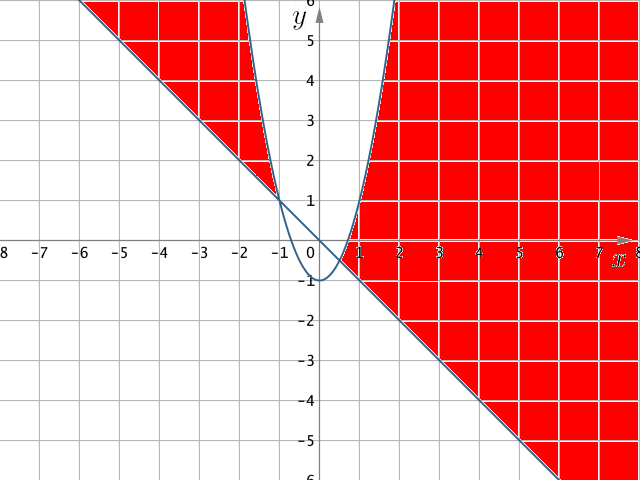
\includegraphics[width=0.7\textwidth]{img/UGlsystmit2.png}
\end{center}

Der markierte Bereich stellt den Lösungsbereich dar. \\
Die Punkte auf den Funktionen selbst sind nicht im Lösungsbereich enthalten. \\
Für den Bereich $ -1 \ \leq \ x \ \leq \ \frac 1 2 $ existiert keine Lösung. \\
Für alle anderen Werte von $x$ sind alle Punkte für die die Bedingung
$ 2x^2 \ - \ 1 \ > \ y \ > \ -x $ erfüllt ist in der Lösungsmenge enthalten.

\section{Quellen} 

\begin{itemize}
\item http://ilias.tfh-wildau.de/~laborwww/downloads/Kap2 \_ komplett.pdf
\item Wikipedia: Lösen von Ungleichungen
\item ftp://ftp.fernuni-hagen.de/pub/fachb/mathe/alggeo/ \linebreak schulte/1011C3.pdf
\end{itemize}
